Our first example of a use case that can be implemented using the matching library is the identification of the best column
match between two dataframes.
In other words, if we have a subject dataframe A and a target dataframe B, we want to find, for each column in A, the most
similar column in B\@.
Why is this relevant for our project?
One of our goals is to extract enough information from a dataset that it can be understood by data analysts and inserted
correctly into data visualization software, to produce relevant graphs and diagrams.
Inserted correctly means knowing which dataframes should go together in the same picture, what columns should be placed
on which axis, and what comparisons are worthy of showcasing in a presentation.
Our tool will be capable of providing suggestions for significant pairs of columns between two or more dataframes, that
should be investigated further.

Towards this end, we must first load the two dataframes (A and B) and their respective metadata (if not available, we generate
them) into memory.
Then, for each column in A, we loop through the columns in B and apply a number of matching algorithms.
Because of the modular nature of our matching library, this list can be edited to the preferences of the user, but in order
to balance accuracy and performance, we have chosen the following:

\begin{itemize}
    \item longest common subsequence of the column names
    \item Levenshtein distance between the column names
    \item matching data types
    \item similarity of the continuity percentages
    \item similarity of the numerical percentages
    \item number of identical values
\end{itemize}

These algorithms produce similarity percentages, which we then average.
Additionally, we calculated the differences of the minimum, maximum, and average values in the columns, where applicable.
Then, we normalized the results, using the following formula:

normalized\_value = (1 - (value - min\_value) / (max\_value - min\_value)) * 100

This way, every difference will be expressed as a similarity percentage.
The lower the difference, the higher the percentage.
We add these percentages to the final average and return the column with the best score.

To apply this algorithm on an example, we will use two dataframes from Kaggle containing the results of a survey of the
state of global happiness in 2015 and 2016, respectively~\cite{kaggleWorldHappinessReport}.
These two dataframes are similar, with the expection of a few columns which are only found in one of them.
A column named ``Standard Error'' only exists in the 2015 report, while two columns named ``Lower Confidence Interval'' and
``Upper Confidence Interval'' only appear in the 2016 report.
These names are not very suggestive, so we will use our tool to try and figure out which other column they relate to (if any).

\begin{figure}[h]
    \centering
    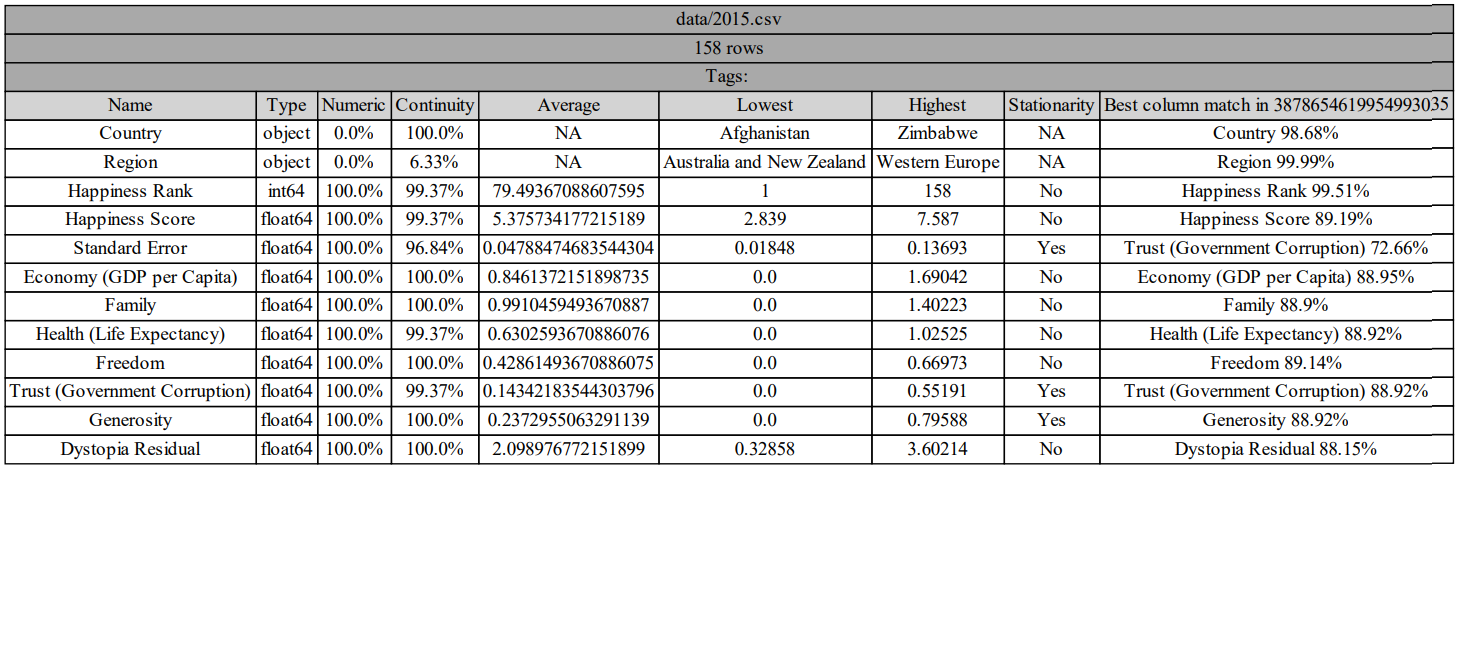
\includegraphics[width=12cm]{figures/best_column_match_id/2015_column_match}
    \caption{Best column matches for the 2015 report}
    \label{fig:2015_column_match}
\end{figure}

\begin{figure}[h]
    \centering
    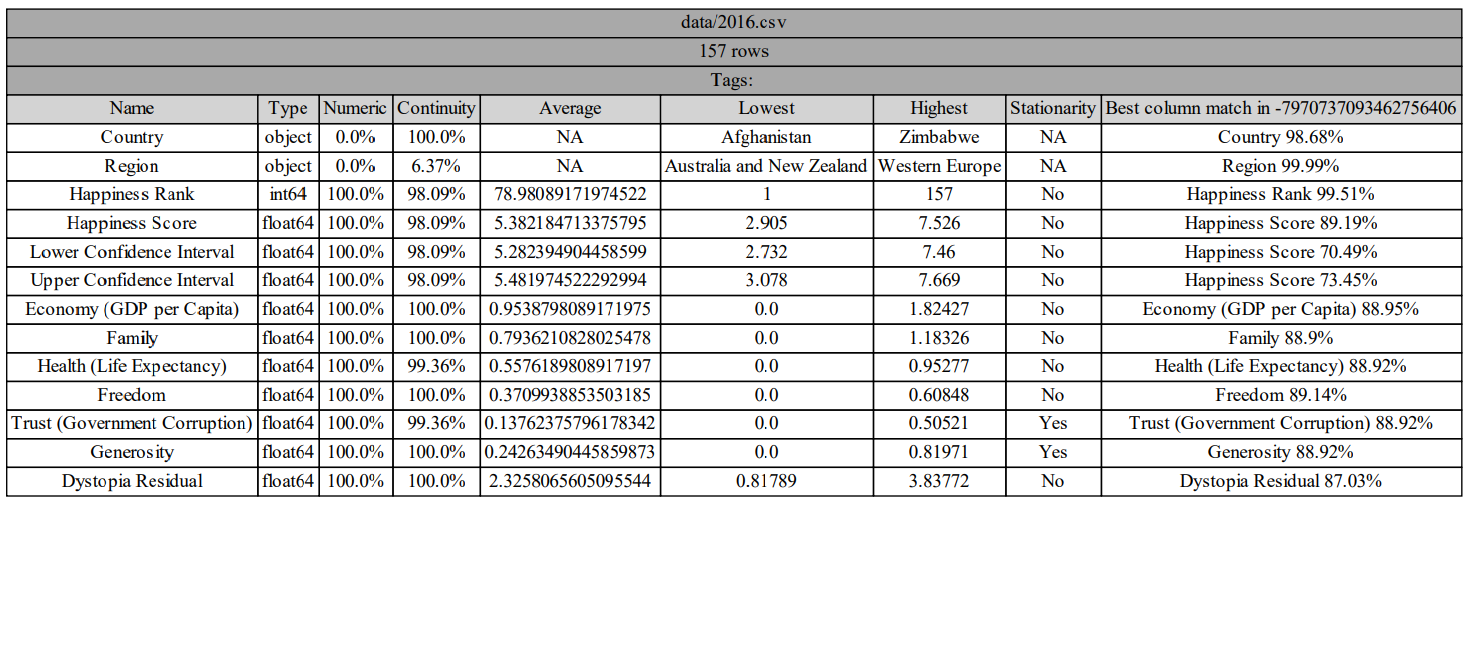
\includegraphics[width=12cm]{figures/best_column_match_id/2016_column_match}
    \caption{Best column matches for the 2016 report}
    \label{fig:2016_column_match}
\end{figure}

First of all, we observe that all columns containing the same information (but for different years), such as Country, Region,
and Happiness Rank have been matched correctly, with high confidence percentages.
In the 2016 report, the two outlier columns have both been matched to the Happiness Score.
We can infer from this that the confidence intervals relate to the accuracy of the happiness score.
This result is verified by the information on Kaggle~\cite{kaggleWorldHappinessReport}.
However, for the 2015 report, the outlier column (``Standard Error'') has been matched to the ``Trust (Government Crruption)''
column.
This is incorrect, as Kaggle tells us the standard error also refers to the happiness score~\cite{kaggleWorldHappinessReport}.
This mistake suggests both that the algorithm can be improved and that these results are merely suggestions, and that at least
some minimal verification is required.
Our design decision for the modularity of the matching library is useful once again, as algorithms can easily be plugged in
and out of use cases such as the best column match identification, in order to verify if the results remain the same.
As a final note on this topic, the metadata column where we store the results of the column matches contains the hash of
the dataframe where the lookup was performed.
This is a unique identifier in the system and ensures the integrity of the metadata.